\documentclass{article}

\author{Angus Griffith}
\title{Summer Research Scholarship Report}

\usepackage{url}
\usepackage{tikz}
\usepackage{fullpage}
\usepackage{amsmath}

\begin{document}
\section{Weyl Formula}
The number of eigenvalues of wavelength in the interval $[0,k]$ is given by the Weyl formula
\begin{equation}
C^w_{0,k} = \frac{\mbox{Area}}{4 \pi} k^2 - \frac{\mbox{Perimeter}}{4 \pi} k + o(XXX)
\end{equation}
We thus dedcuce that the number of eigenvalues in the interval $[k_a, k_b]$ is given by
\begin{equation}
C^w_{k_a,k_b} = \frac{\mbox{Area}}{4 \pi} (k_b^2 -k_a^2) - \frac{\mbox{Perimeter}}{4 \pi} (k_b - k_a) + o(XXX)
\end{equation}
\section{Upper and Lower Bounds for Normal Derivatives of Dirichlet Eigenfunctions}
\cite{HT02}

\section{Upper and Lower Bounds for Boundary Values of Neumann Eigenfunctions}
\cite{BHXX}

\section{Boundary Quasi-Orthogonality and sharp inclusion bounds for large Dirichlet Eigenvalues}
\cite{BH11}

\section{Fast computation of high-frequency Dirichlet eigenmodes}
\cite{BH14}

\section{Examples: Dirichlet eigenvalues}
\paragraph{}
In this section we present a numerical investigation of three methods used to compute Dirichlet eigenvalues.
The computation is performed with the MATLAB toolbox mpspack \cite{MPS}.
\begin{figure}[htbp]
\centering
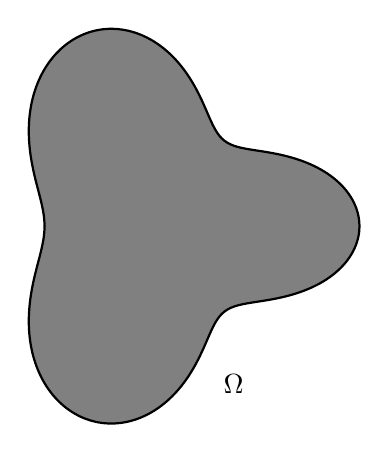
\begin{tikzpicture}[scale=2]
  \draw[thick,smooth, domain=0:2*pi,fill=gray,samples=200] plot (
        xy polar cs:angle=\x r, radius={1+0.3*cos(deg(3*\x+0.6*sin(deg(\x))))}
    );
  \node at (0.5,-1) {$\Omega$};
\end{tikzpicture}
\caption{The non-symmetric, smooth domain $\Omega$.}
\end{figure}
We construct a domain $\Omega$ from the region enclosed by the parametric function
\[
\theta \mapsto (\theta, 1 + 0.3 \cos( 3 \theta + 0.6 \sin \theta))
\]
in polar coordinates, for $\theta \in [0, 2\pi)$.
We are interested in computing eigenvalues $k^2_j$ of the Dirichlet Laplacian. That is, \\
\begin{align*}
(\Delta + k_j^2) \phi_j = 0 & \quad \mbox{in } \Omega, \\
\phi_j  = 0 & \quad \mbox{on } \partial \Omega.
\end{align*}
where $\phi_j$ are the associated eigenfunctions.
\paragraph{}
We discretise the boundary into $N$ evenly spaced points and search for the $k_j$.
Since $\Omega$ is non-symmetric the multiplicity of each eigenvalue will be one.
The following is a comparison of the performance of the various methods built into mpspack.
Each calculation is repeated 5 times and an average is taken.
\paragraph{}
We plot the time taken to search for the eigenvalues as a function of $k$ and $N$.
The number of eigenvalues found $N_{k,k+1}$ is compared to the number expected $C^w_{k,k+1}$ by the Weyl formula \ref{weyl}.
The colour of the plot is given by $|C_{k,k+1} - C^w_{k,k+1}|$.
\subsection{Neumann-to-Dirichlet method}
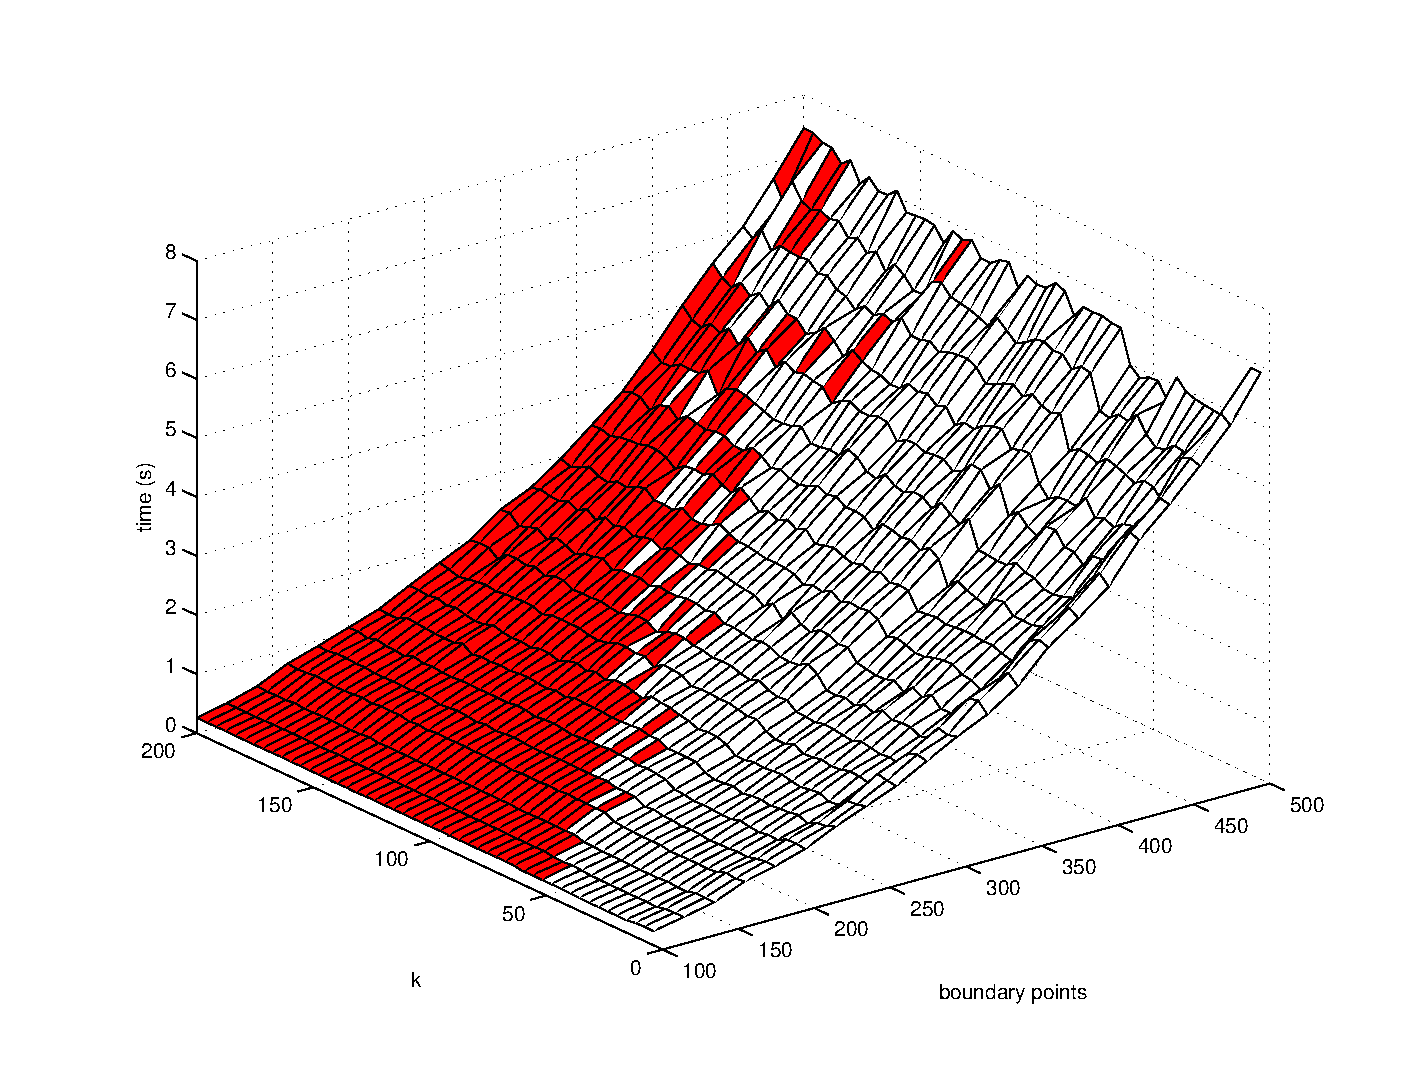
\includegraphics[width=0.9\textwidth]{dtn.eps} \\
Observe that the expected $O(N^2)$ growth in the runtime is clear.
We also observe a small but significant growth in the runtime as $k$ increases for fixed $N$.
\subsection{Fredholm determinant method}
\subsection{Method of particular solutions}

\begin{thebibliography}{9}

\bibitem[HT02]{HT02}
Hassell. A and Tao, T.
\textsl{Upper and lower bounds for boundary values of Neumann eigenfunctions}.
Math. Res. Lett. Vol. 9 (3), 2002. % 289 -- 305

\bibitem[BH]{BHXX}
Barnett, A.H. and Hassell. A.
\textsl{Upper and lower bounds for boundary values of Neumann eigenfunctions}.
In preparation, 2015.

\bibitem[BH11]{BH11}
Barnett, A.H. and Hassell, A.
\textsl{Boundary quasi-orthogonality and sharp inclusion bounds for large Dirichlet eigenvalues}.
SIAM J. Numer. Anal. Vol. 49 (3), 2011.

\bibitem[BH14]{BH14}
Barnett, A.H. and Hassell, H.
\textsl{Fast Computation of High-Frequency Dirichlet Eigenmodes via Spectral Flow of the Interior Neumann-to-Dirichlet Map}.
Comm. Pure Appl. Math. Vol 67, 2014.

\bibitem[MPSpack]{MPS}
Barnett A. and Betcke T.
mpspack,
\textsl{A MATLAB toolbox to solve Helmholtz PDE , wave scattering and eigenvalue problems using particular solutions and integral equations},
Version 1.33-dev, 2014.
Available online: \url{https://code.google.com/p/mpspack/}

\end{thebibliography}
\end{document}
